% !TeX root = ../Book1.tex
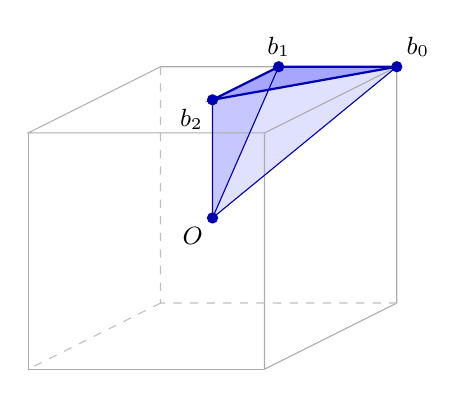
\begin{tikzpicture}[font=\small,scale=1.2]
	\coordinate (O) at (0,0);
	\coordinate (A) at (1.95,1.6);
	\coordinate (B) at (-.55,1.6);
	\coordinate (C) at (-1.95,.9);
	\coordinate (D) at (.55,.9);
	\coordinate (a) at (1.95,-.9);
	\coordinate (b) at (-.55,-.9);
	\coordinate (c) at (-1.95,-1.6);
	\coordinate (d) at (.55,-1.6);
	\coordinate (M) at (.7,1.6);
	\coordinate (F) at (0,1.25);
	\fill[blue!12] (O)--(A)--(M)--cycle;
	\fill[blue!22] (O)--(M)--(F)--cycle;
	\fill[blue!35] (A)--(M)--(F)--cycle;
	\draw[gray!65] (A)--(B)--(C)--(D)--cycle;
	\draw[gray!65] (A)--(a)--(d)--(D);
	\draw[gray!65] (C)--(c)--(d);
	\draw[gray!50,dashed] (B)--(b)--(a) (b)--(c);
	\draw[blue!70!black,thick] (A)--(M)--(F)--cycle;
	\draw[blue!70!black] (O)--(A) (O)--(M) (O)--(F);
	\foreach \p in {O,A,M,F} {\fill[blue!70!black] (\p) circle (1.7pt);}
	\node[below left] at (O) {\(O\)};
	\node[above right] at (A) {\(b_0\)};
	\node[above] at (M) {\(b_1\)};
	\node[below left] at (F) {\(b_2\)};
\end{tikzpicture}
